\section{SSLStrip+}

\begin{frame}{Fonctionnement de HSTS}

\end{frame}

\begin{frame}{Attaque SSLStrip+}
  - création d'un faux nom de domaine
  - Ressemblance avec le vrai nom de domaine
  - Remplacement des URL sécurisés par la fausse URL
  - Le navigateur va faire une requête DNS sur le faux domaine
  - L'attaquant doit contrôler la requête
  - SSLStrip peut alors fonctionner
\end{frame}

\begin{frame}{Attaque SSLStrip+}
    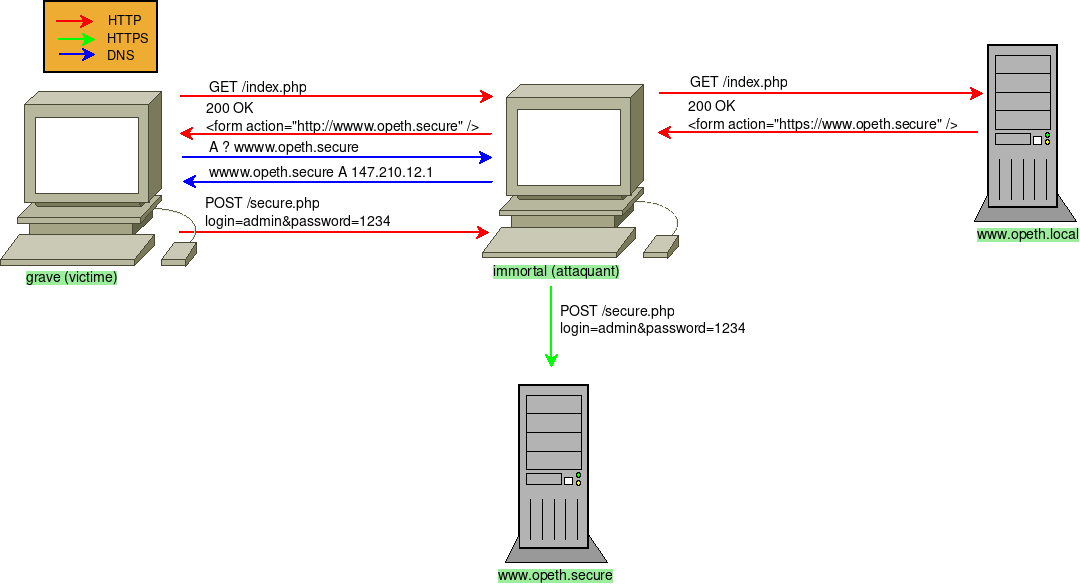
\includegraphics[width=\linewidth]{../medias/sslstrip2/attack.png}
\end{frame}
